%%%%%%%%%%%%%%%%%%% EJERCICIO 12 %%%%%%
\textbf{Ejemplo 12}\\
Una deuda de 15.000 COP fue contraída hace 2 meses con fecha de vencimiento en 4
meses a partir de hoy, esta posee un interés del 24\% nominal anual trimestre vencido y
otra deuda de 25.000 COP contraída hace un mes con vencimiento de 8 meses a partir de hoy
e intereses del 28\% nominal anual semestre vencido. Se van a cancelar las deudas
mediante dos pagos de igual valor, efectuados el primero el día de hoy y el segundo en 6
meses. Con un interés del 30\% nominal anual mes vencido,
determinar el valor de los pagos.\\ \\
%\newpage %USAR SOLO SI EL SOLUCIÓN QUEDA SOLO Y ES NECESARIO BAJARLO A LA SIGUIENTE PAGINA
\textbf{Solución.}\\
%La tabla ira centrada
\begin{center}
  \renewcommand{\arraystretch}{1.5}% Margenes de las celdas
  %Creación de la cuadricula de 3 columnas
  \begin{longtable}[H]{|C{0.3\linewidth}|C{0.3\linewidth}|C{0.35\linewidth}|}
    %Creamos una linea horizontal
    \hline
    %Definimos el color de la primera fila
    \rowcolor[HTML]{FFB183}
    %%%%% INICIO ASIGNACIÓN PERíODO FOCAL %%%%%%%
    %%%%%%%%%% INICIO TITULO
    %Lo que se hace aquí es mezclar las 3 columnas en una sola
    \multicolumn{3}{|c|}{\cellcolor[HTML]{FFB183}\textbf{1. Asignación período focal}}                                                                                              \\ \hline
    \multicolumn{3}{|c|}{\textbf{ $pf : \textit{ período focal: 6 pmv} $}}                                                                                                          \\ \hline
    %%%%%%%%%% FIN TITULO
    %%%%% INICIO DECLARACIÓN DE VARIABLES %%%%%%%
    %%%%%%%%%% INICIO TITULO
    %Lo que se hace aquí es mezclar las 3 columnas en una sola
    \multicolumn{3}{|c|}{\cellcolor[HTML]{FFB183}\textbf{2. Declaración de variables}}                                                                                              \\ \hline
    %%%%%%%%%% FIN TITULO
    \multicolumn{3}{|c|}{\cellcolor[HTML]{FFB183}\textbf{Deuda 1}} \\ \hline
    \multicolumn{1}{|c|}{\cellcolor[HTML]{FFB183}\textbf{Valores monetarios}} &
    \multicolumn{1}{|c|}{\cellcolor[HTML]{FFB183}\textbf{Valores no monetarios}} &
    \multicolumn{1}{|c|}{\cellcolor[HTML]{FFB183}\textbf{Incógnitas}} \\ \hline
    %Valores de las variables
    $P_{1} = 15.000 $ COP & $i_{1} = 6\% \textit{ ptv} $  & $F_{1} =   P_{1}i_{1} $ COP  \\
    & $n_ {1} = 2 \textit{ ptv} $ & $F_{3} = ? $ COP \\
    & $j_{1} = 24\% \textit{ natv} $ & \\
    &  & \\
    \hline
    %Sección 2.2
    \multicolumn{3}{|c|}{\cellcolor[HTML]{FFB183}\textbf{Deuda 2}} \\ \hline
    \multicolumn{1}{|c|}{\cellcolor[HTML]{FFB183}\textbf{Valores monetarios}} &
    \multicolumn{1}{|c|}{\cellcolor[HTML]{FFB183}\textbf{Valores no monetarios}} &
    \multicolumn{1}{|c|}{\cellcolor[HTML]{FFB183}\textbf{Incógnitas}} \\ \hline
    %Valores de las variables
    $P_{2} = 25{.}000 $ COP & $j_{2} = 28\% \textit{ nasv} $  & $F_{2} = ? \textit{ COP} $ \\
    & $m_{2} = 2 \textit{ ptv} $ & $F_{3} = ? \textit{ COP} $ \\
    & $i_{2} =\frac{28\% \textit{ nasv}}{2 \textit{ psv}} = 14\% \textit{ psv} $ & \\
    & $n_ {2} = 1.5 \textit{ psv}$ & \\ \hline
    %Sección 2.2
    \multicolumn{3}{|c|}{\cellcolor[HTML]{FFB183}\textbf{Deuda equivalente}} \\ \hline
    \multicolumn{1}{|c|}{\cellcolor[HTML]{FFB183}\textbf{Valores monetarios}} &
    \multicolumn{1}{|c|}{\cellcolor[HTML]{FFB183}\textbf{Valores no monetarios}} &
    \multicolumn{1}{|c|}{\cellcolor[HTML]{FFB183}\textbf{Incógnitas}} \\ \hline
    %Valores de las variables
    & $j_{3} = 30\% \textit{ namv} $  & $F_{3} = F_{6} = ? \textit{ COP} $ \\
    & $m_{3} = 12 \textit{ pmv} $ & \\
    & $i_{3} =\frac{30\% \textit{ namv}}{12 \textit{ pmv}} = 2.5\% \textit{ psv} $ & \\
    & $n_{3} = 6 \textit{ psv}$ & \\ \hline
    %%%%% FIN DECLARACIÓN DE VARIABLES


    %%%%% INICIO FLUJO DE CAJA
    \rowcolor[HTML]{FFB183}
    \multicolumn{3}{|c|}{\cellcolor[HTML]{FFB183}\textbf{3. Diagrama de flujo de caja}}                                                                                             \\ \hline
    %Mezclamos 3 columnas y pondremos el dibujo
    %%%%%%%%%%%%% INSERCIÓN DE LA IMAGEN
    %Deberán descargar las imágenes respectivas del drive y pegarlas en la carpeta
    %n_capitulo/img/ejemplos/1/capitulo1ejemplo1.pdf  (el /1/ es el numero del ejemplo)
    \multicolumn{3}{|c|}{ 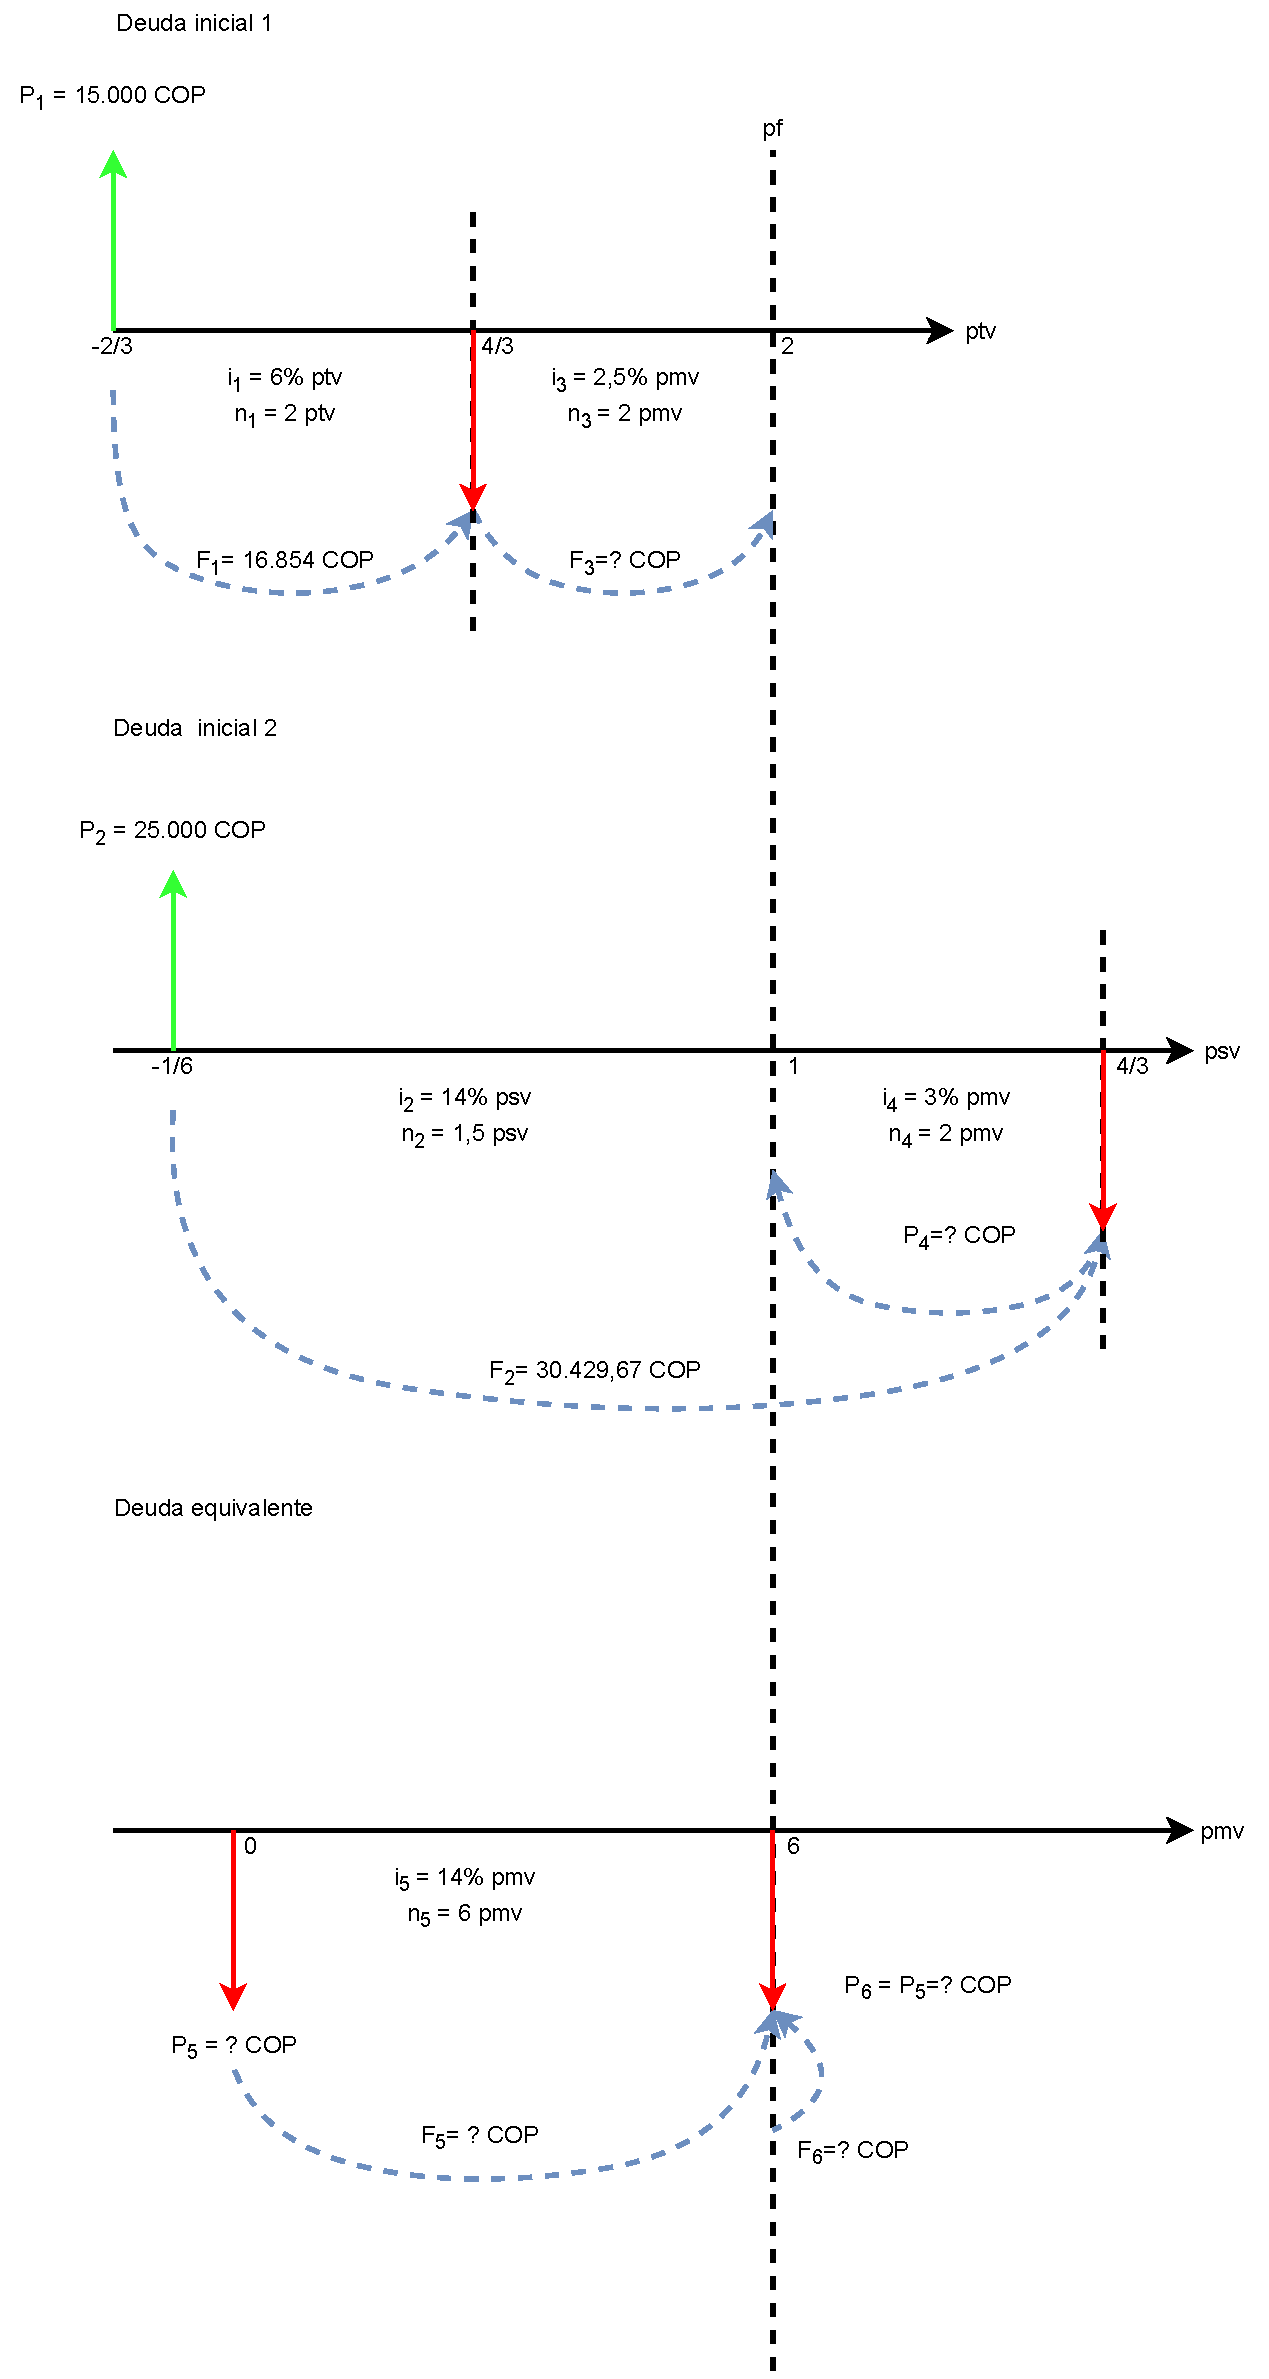
\includegraphics[trim=-5 -5 -5 -5 , scale=0.4]{2_Capitulo/img/ejemplos/14/Ejemplo 12Ver.pdf}}
    \\ \hline
    %%%%%%%%%%%%% FIN INSERCIÓN DE IMAGEN
    %%%%%FIN FLUJO DE CAJA



    %%%%% INICIO DECLARACIÓN FORMULAS
    %%%%%%%%%%% INICIO TITULO
    \rowcolor[HTML]{FFB183}
    \multicolumn{3}{|c|}{\cellcolor[HTML]{FFB183}\textbf{4. Declaración de fórmulas}}                                                                                               \\ \hline
    %%%%%%%%%%% FIN TITULO
    %%%%%%%%%%% INICIO MATEMÁTICAS

    $F = P(1+i)^n \hspace{0.3cm} \textit{Valor futuro}$
    & \multicolumn{2}{c|}{$F_{3}+P_{4}=F_{5}+P_{6}\hspace{0.3cm}\textit{Ecuación de valor}$}
    \\
    $j=im\hspace{0.3cm}\textit{Tasa periódica anualizada}$
    & \multicolumn{2}{c|}{$P = F(1+i)^{-n} \hspace{0.3cm} \textit{Valor presente}$ }
 
    \\ \hline

    %%%%%%%%%% FIN MATEMÁTICAS
    %%%%%% INICIO DESARROLLO MATEMÁTICO
    \rowcolor[HTML]{FFB183}
    %%%%%%%%%%INICIO TITULO
    \multicolumn{3}{|c|}{\cellcolor[HTML]{FFB183}\textbf{5. Desarrollo matemático}}                                                                                                 \\ \hline
    %%%%%%%%%% FIN TITULO
    %%%%%%%%%% INICIO MATEMÁTICAS
    \multicolumn{3}{|c|}{$F_{1}= 15{.}000$ COP $ (1 + 0.06)^{2}=  16{.}854 \textit{ COP}$} \\
    \multicolumn{3}{|c|}{$F_{2}= 25{.}000$ COP $ (1 + 0.14)^{1.5}= 30{.}429.67 \textit{ COP}$} \\ 
    \multicolumn{3}{|c|}{$16{.}854$ COP$ (1+0.025)^{2} + 30{.}429.67\textit{ COP} (1+0.025)^{-2}$} \\
    \multicolumn{3}{|c|}{$ = P_{5}(1+0.025)^{6} + P_{5}$} \\
    \multicolumn{3}{|c|}{$46{.}670.63\textit{ COP} = P_{5} ((1.025)^{6} + 1)$} \\
    \multicolumn{3}{|c|}{$\frac{46{.}670.63\textit{ COP}}{(1.025)^{6} + 1} = P_{5}$} \\
    \multicolumn{3}{|c|}{$P_{5}=21{.}609.84\textit{ COP}$} \\ \hline

    %%%%%%%%%% FIN MATEMÁTICAS
    %%%%%% FIN DESARROLLO MATEMÁTICO
    %%%%%% INICIO RESPUESTA
    \rowcolor[HTML]{FFB183}
    %%%%%%%%%%INICIO TITULO
    \multicolumn{3}{|c|}{\cellcolor[HTML]{FFB183}\textbf{6. Respuesta}}                                                                                                             \\ \hline
    %%%%%%%%%% FIN TITULO
    %%%%%%%%%% INICIO RESPUESTA MATEMÁTICA
    \multicolumn{3}{|c|}{{$F_{5}$ = $F_{6}$ = 21.609,84 COP.}}                                                                                                                                                                               \\ \hline


    %%%%%%%%%% FIN MATEMÁTICAS
    %%%%%% FIN RESPUESTA
  \end{longtable}
  %Se crean dos lineas en blanco para que no quede el siguiente texto tan pegado
  %\newline \newline %USARLO SI CREES QUE ES NECESARIO
\end{center}
%%%%%%%%%%%%%%%%%%%%%%%%%%FIN EJERCICIO 12 %%%%%%%%%%%%%%%%%%%%%%%%%%%
\setlength{\parskip}{\baselineskip}
